%!TEX root = ../template.tex
%%%%%%%%%%%%%%%%%%%%%%%%%%%%%%%%%%%%%%%%%%%%%%%%%%%%%%%%%%%%%%%%%%%%
%% chapter3.tex
%% NOVA thesis document file
%%
%% Chapter with a short latex tutorial and examples
%%%%%%%%%%%%%%%%%%%%%%%%%%%%%%%%%%%%%%%%%%%%%%%%%%%%%%%%%%%%%%%%%%%%

\typeout{NT FILE chapter3.tex}%

\chapter{State of the Art}
\label{cha:stateofart}

In this Chapter, an extensive delivery of the existing works regarding the main topics covered in this thesis are presented. This will include (1) existing works for information retrieval in time series, mainly in terms of event detection and segmentation, (2) approaches for summarization of time series, (3) symbolic representation techniques and how these can be used for (5) classification tasks and (6) query-based search mechanisms.

\section{Novelty, Periodicity and Similarity Search on Time Series} % (fold)
\label{sec:if_timeseries}


Prior works in information retrieval, most specifically in novelty, periodicity and similarity search (event detection), focus on change point detection or segmentation, where the strategies are categorized as online versus offline, univariate versus multivariate, model-based versus non-parametric and unsupervised versus supervised \cite{cpd_alan, review_1, review_2}. We will further explore the existing literature in supervised and unsupervised methods for this purpose. In addition, as the proposed approaches rely on the usage of a \gls{ssm}, the currently available knowledge on the \gls{ssm} for the same tasks are explained.

\subsection{Supervised Methods}

Supervised methods include multi-class, binary and virtual classifiers optimized to detect change points \cite{review_1}, where the nature of the change can be provided as an additional advantage. Another example uses neural networks with transfer learning for segmentation \cite{pedromatias}. Subsequence search might also be a potential method given a well-selected pattern \cite{folgado2022tssearch}. However, supervised methods rely upon brittle training sets and class imbalance, since there are more in-state sequences than change point sequences \cite{review_1}. An additional problem reported by \cite{cpd_alan} is that most algorithms' performance was validated in synthetic data, where the given nature of the application was not optimal. In response, a benchmark is available for change point detection \cite{cpd_alan}, where methods can be compared on real data. This study applies this benchmark as a reference of state-of-the-art methods.

\subsection{Unsupervised Methods}

Existing classic non-supervised methods in change point detection,  such as \textit{Bayesian Online Change Point Detection} (BOCPD) \cite{bocpd}, \textit{Binary Segmentation} (BINSEG) \cite{binseg} and \textit{Segmentation Neighbourhood} (SegNeigh) \cite{segneigh}, are witnessed to be able to perform in state-of-the-art applications from various domains \cite{cpd_alan}. However, BOCPD needs hyperparameter tuning for sound performance, while BINSEG and SegNeigh have not been used in multidimensional domains. Besides, these methods have not been reported to cope with a multi-timescale change \cite{cpd_alan}. The available repository \cite{cpd_alan} collecting the implementation of some offline methods \cite{review_2} reported above lacks a visual output that can provide users with the location of the change points. Another method applicable to real data domains, called \textit{Fast Low-cost Online Semantic Segmentation} (FLOSS) \cite{eamonn1, eamonn_segmentation}, searches regime changes based on the nearest neighbours of subsequences, which allows the similarity comparison between segments for the segmentation and summarization of long-term time series.

Several works that use unsupervised methods are found for the identification of cyclic information and anomalies. An automated algorithm of segmentation was able to separate complex and multidimensional data into smaller segments that can be described through harmonic models. This algorithm revealed to be significantly useful to identify cyclic movement without any \textit{a priori} knowledge of the input data, using a combination of a recursive least squares segmentation algorithm, a model fitting of damped harmonics, and in the end, a clustering analysis to classify the events \cite{Lu2004,Lu2003}. The usage of features is of great relevance in unsupervised works, and methods are found to select adequate features for detection and classification tasks, such as in ~\cite{machado2015}. Another example is the use of four-pass UKF (unscented Kalman filter) to produce an unified model with kinematic parameters. These may then be segmented by analyzing the parameter's zero crossing velocity and in the end uses a clustering algorithm to identify repetitive segments \cite{Wang2015a}. Other methods rely on a self-similarity approach, namely in the work of \textit{Neuza et. al}\cite{neuza}, where cyclic information is segmented by searching for minimums, in the convolution of a segment of the signal with itself. The \textit{Matrix Profile (MP)}, which is a method that compares all sub-sequences of a given time series with themselves through the \gls{ed} and returns the minimum value for each distance profile. This method highlights the moments of the time series which are similar within themselves \cite{Yeh2018}, being then used for a mutltitude of purposes in time series data mining \cite{mpdist, mpxxiv, mpxix, mpxvi}. Additionally, autocorrelation revealed itself an useful tool, as the search over maximum values can infer the cyclic nature of the data \cite{Bauters2014}. Finally, for anomaly detection in industrial scenarios, \textit{Varandas et. al} applies an unsupervised method based on the clustering of time series segments to detect the execution of improper movements \cite{Varandas19}. 

\subsection{Self-Similarity Matrix (SSM)}

Similarity matrices have been used for the analysis of time series in the past. These matrices have several representations and denominations, being the most commonly known \textit{recurrence plot}. These plots are a similarity matrix thresholded by a specific value that highlight only similar regions. The representation of these maps was used to analyze time series \cite{eamonn_dotplots,recurrenceplots1} and search for reoccurring shapes, anomalies or symmetric behaviors \cite{eamonn_dotplots}. It was also used for time series classification by inputting the recurrence plot into a neural network (Convolutional Neural Networks) \cite{recurrenceplots1, recurrenceplots2} or forecasting \cite{recurrenceplots3}.

The \gls{ssm} has more information than the recurrence plot (which has been thresholded). Several usages have been explored in the audio domain, namely for segmentation, thumbnailing, periodiciy search or music alignment. For this, the audio signal is transformed on a feature-based representation \cite{fmp1, fmp2}. 
The \gls{ssm} has been used for segmentation in the audio domain, based on a feature representation of the audio signal \cite{fmp1, fmp2}. The advantage of the \gls{ssm} is that it provides a considerable amount of information for a specific timescale. This study promotes \gls{ssm} concepts and applications from the audio domain to other time series domains. The proposed method can detect events with context, associating the estimated events with patterns, (dis)similarities, periodicity and novelty, and a possible extension is the task of summarization. The search mechanism is primitively based on a specific timescale and can evolve recursively to perform multi-timescale searches.

\subsection{Summarization}
\label{sec:literature_summarize}

Very few strategies are found to make compact and meaningful representation of time series. The works that can be highlighted refer to time \textit{snippets} and time series \textit{bitmaps} \cite{snippets, bitmap}. The first highlights the limitation of current methods in providing a satisfactory solution to time series \textit{summarization}. It proposes a method that is able to segment the \textit{k} most \textit{representative} sub sequences of a time series, and use these elements as the summary. This strategy answers the segmentation and similarity. Regarding the time series \textit{bitmap} representation, the strategy is able to provide a coded bitmap with information on cluster, anomaly and other regularities on data collection. These bitmaps were used as folder icons, and also answer several of the aforementioned characteristics, such as \textit{similarity} and \textit{events}. An example of both strategies can be seen on Figure \ref{fig:keogh_strat}.

\begin{figure}[t]
    \centering
    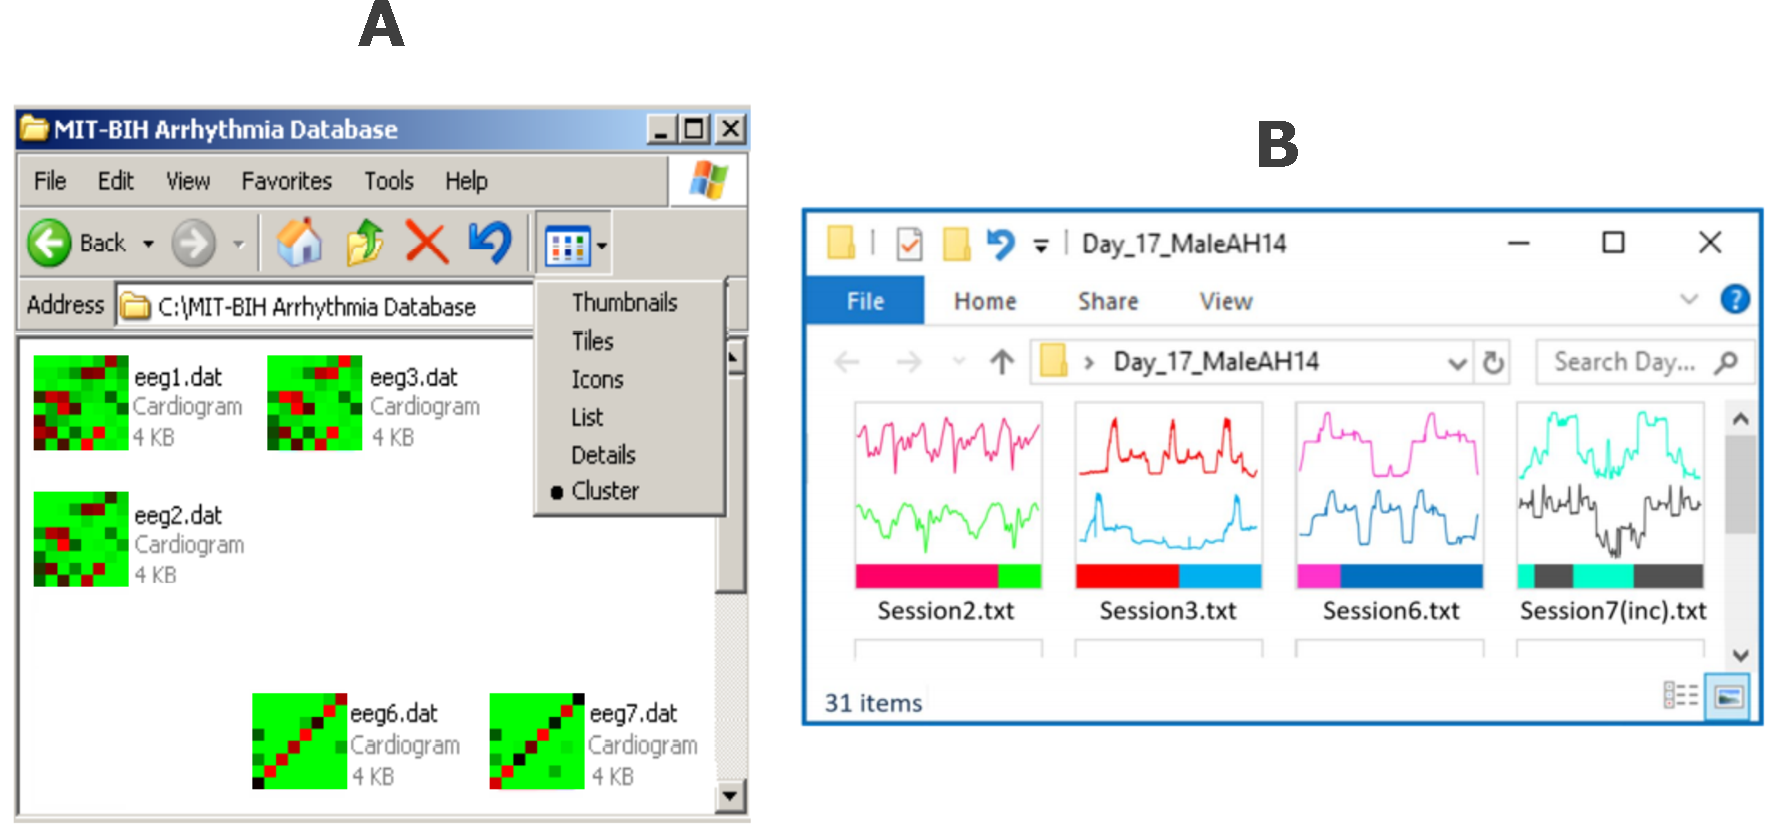
\includegraphics[width=0.8\linewidth]{keogh_examples.pdf}
    \caption{Strategies for time series summary found on the literature. These images are taken from the works from \cite{snippets, bitmap}}
    \label{fig:keogh_strat}
\end{figure}

Time series \textit{shapelets} are also a method that could provide interesting results. However, the strategy is \textit{supervised}, and the point of the proposed method is to have \textit{no apriori} knowledge about the structure of the data, except the time scale in which the summarization is performed. 
\par
Other interesting strategies provide a transformation of time series into text and could be used for time series summarization, but are not able to suitably summarize a time series from the textual representation \cite{ssts, sax}.

Strategies that are typically used to present information in a compact way are found in several domains. In text analysis, for instance, the relationship between repeating sequences is illustrated with arc diagrams \cite{bitmap, arcplots}. These show where repeating sequences occur in a very concise way. This has a range of applications that include, for example text and DNA sequence analysis.

\begin{figure}[b]
    \centering
    \begin{subfigure}{0.5\linewidth}
    \centering
        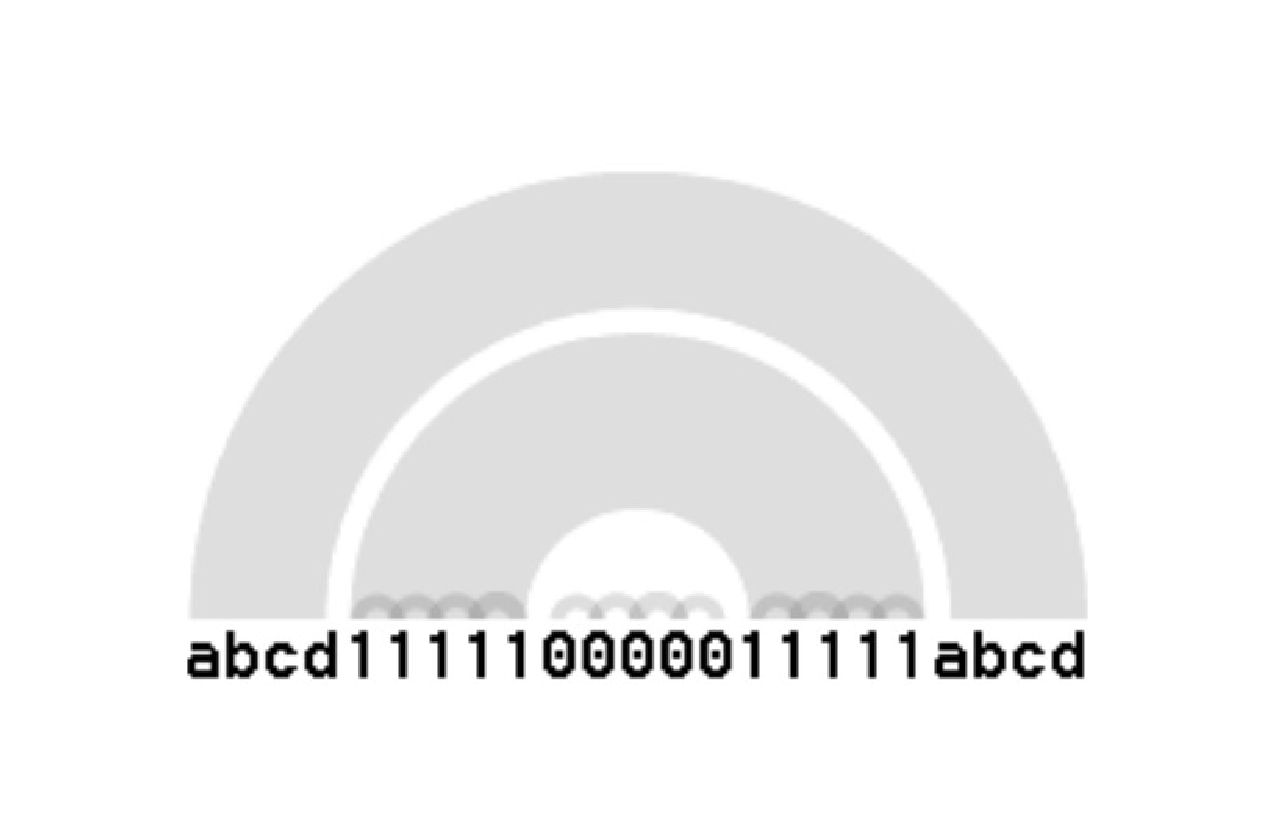
\includegraphics[width=0.9\linewidth]{arcplots.pdf}
        \caption{}
        \label{fig:genomic1}
    \end{subfigure}%
    \begin{subfigure}{0.5\linewidth}
        \centering
        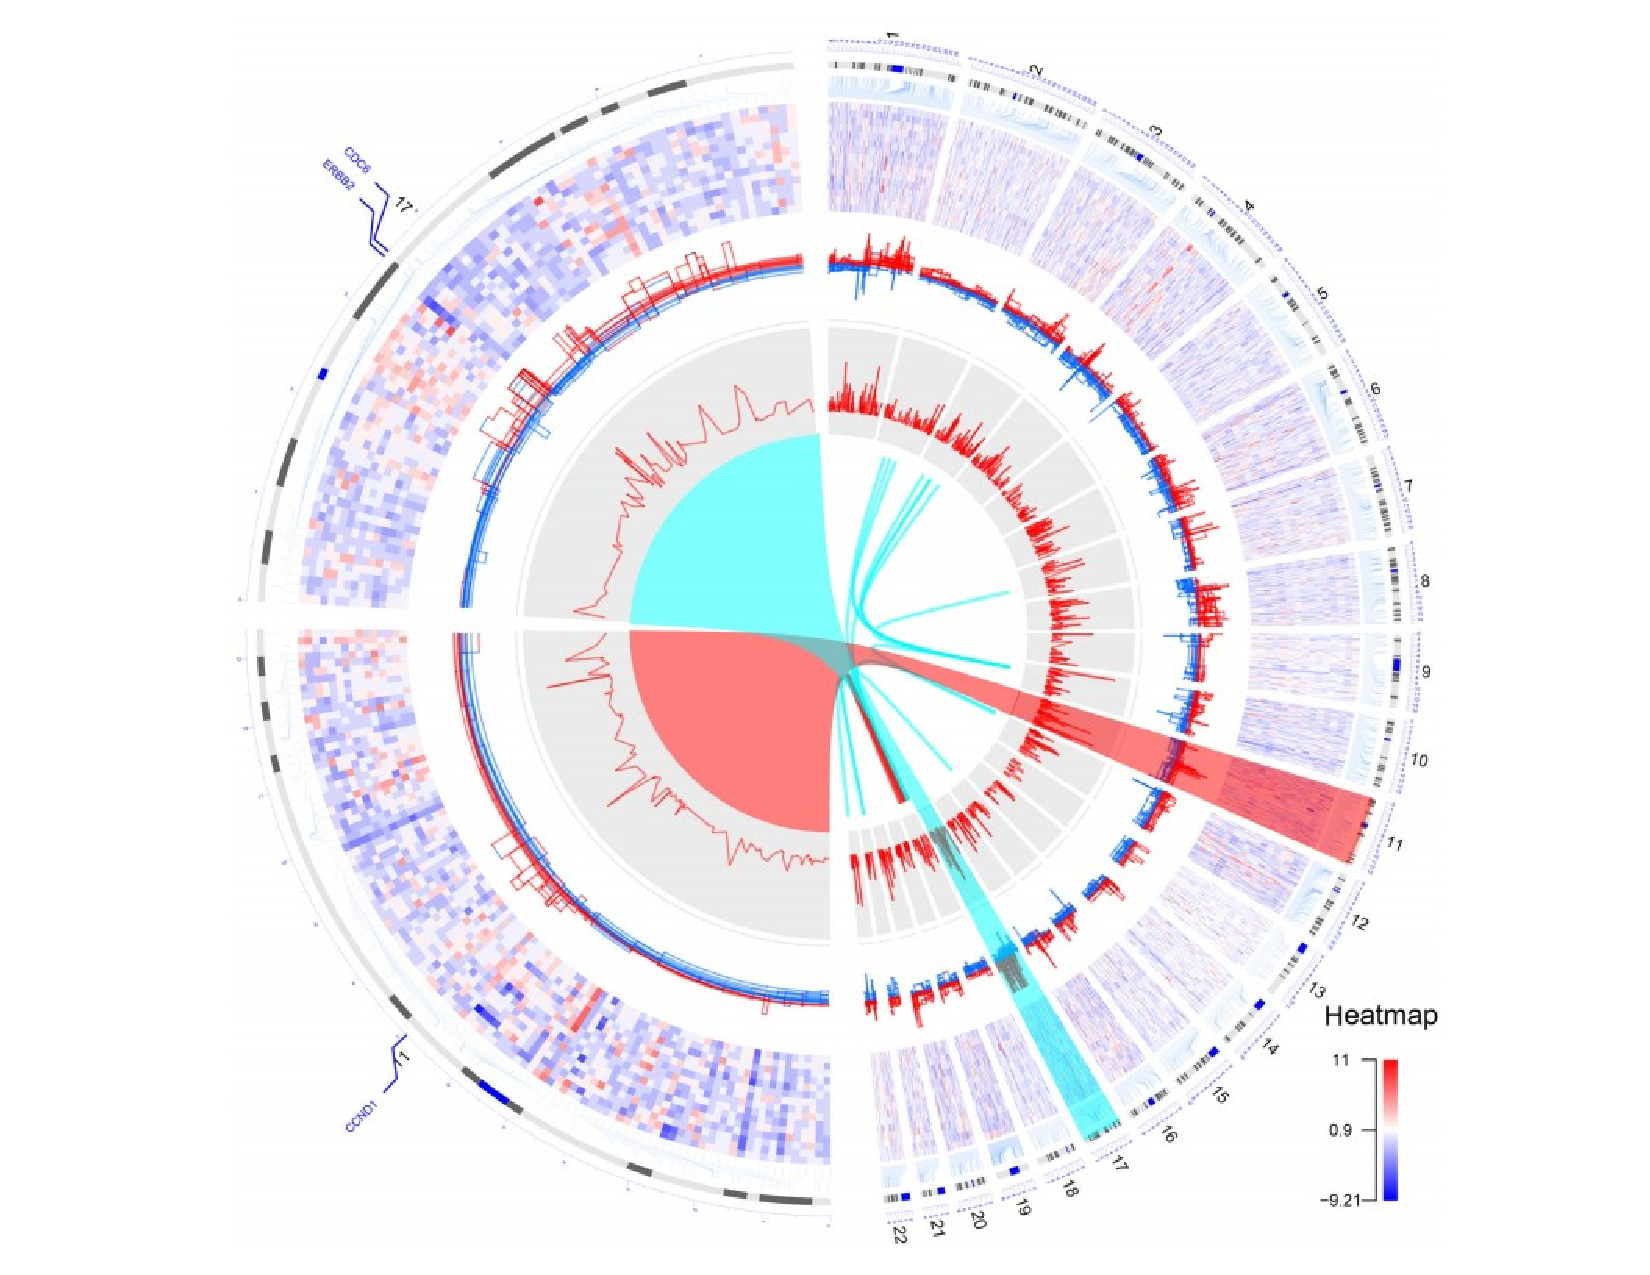
\includegraphics[width=0.9\linewidth]{genomics.pdf}
        \caption{}
        \label{fig:genomic2}
    \end{subfigure}
    \caption{A - Diagram for string association. This image is taken from the works from \cite{arcplots}; B - Circular plot by OmicCircos. Several layers (Circular tracks) identify genome position, expression heatmaps, correlation between expression and CNV, among other features. The image is taken from the works from \textit{Ying Hu, et al.} \cite{genomics}.}
    \label{fig:summary_example}
\end{figure}

One domain that has a particular relevance in data visualization is genomics. Graphical genome maps are found to concatenate a significant amount of information in a very compact way. Genome features and sequence characteristics are assessed with this visual strategy. An example can be found on Figure \ref{fig:genomic2}. This visualization strategy can provide increasing circular layers of information. Although we are used to look at time series from left to right, a circular representation can have benefits to concatenate the information we want to include.
\par
In the musical domain, strategies have also been developed that summarize audio time series with segmentation techniques. One of the strategies that is common to be used involves detecting novelty instances on a similarity matrix representation of the audio signal, called \gls{ssm}. This data structure provides a significant range of information that can be used to retrieve structural information, such as block and periodic structures \cite{fmp1, fmp2, audiolabs1, audiolabs2}. This method will inspire our visualization strategy, which will be explained in a further section.

\section{Text-based representation of time series}

In the field of signal processing, few are the algorithms that rely on syntactic models to solve query search tasks. In the late 60s and 70s, syntactic approaches in time series started to appear, but have fallen into disuse over time and have recently re-emerged.
\par
Some application of these linguistic models into mathematical domains  have been led by T. Pavlidis ~\cite{pavlidis1,pavlidis2} and K. Fu~\cite{kfu7}, which have an exhaustive list of studies in pattern recognition and computer vision fields related with the symbolic description of 2D-shapes. Moreover, \textit{Pavlidis} expressed that the primary problem in the implementation of such methods with functions of one variable would involve the representation of the waveform into a one dimensional string of primitives over a finite alphabet~\cite{pavlidis2}.
\par
These concepts inspired multiple works that have emerged and applied a syntactic approach to pattern recognition tasks. Some examples can be addressed in the field of \gls{ecg} analysis~\cite{Horowitz, Udupa, Skordalakis, DCtnh}. \textit{Horowitz} \textit{et. al.} describe that the detection of peaks in \gls{ecg} signals can be achieved by specifying a set of primitives (one symbol or a group of symbols that represent one sample of the signal) able to be representative of the shape of the \gls{ecg} peaks. The generated string is made by combining the information of the amplitude and the first derivative, which is thereafter parsed based on a set of context free grammar rules. This enables to detect the \gls{ecg} peaks. 
\par
Similar approaches were made in \textit{Skordalakis and Udupa et. al.}, although in these cases, the set of primitives is coded with the length and slope of the line segment~\cite{Udupa,Skordalakis}. The use of symbolic representations has also been found in biometric \gls{ecg} by means of compression techniques~\cite{DCtnh}. 
\par
Recently, approaches based on the symbolic representation of time series have reappeared and provided satisfactory and competitive results in comparison to statistical methods, proving that the use of small sets of primitives and grammatical rules are a possible way of describing large sets of patterns by efficiently representing the signal's structures into an ordered hierarchical sequence of characters.~\cite{Hamdi2017}.
\par
For instance, in the last decade, several works were found in the literature that used symbolic approximation of time-series. Some were found to model finite state automaton from the generation of symbolic time series, which were able to describe the probabilistic flow of data and with this detect patterns on time series\cite{Rajagopalan,Piccardi}. Both \textit{Lin} \textit{et.al.} with the \gls{sax} and \textit{Senin} \textit{et. al.} used grammar based compress methods to detect anomalies by comparing subsequences of the signal~\cite{sax,Senin}. Another similar approach uses a symbolic representation of time series for information retrieval \cite{YueLi2017}. 
\par
In \cite{Ordonez2011}, \textit{Bag-of-words} models are used on a symbolic representation of time series to classify physiological data. Additionally, several works regarding symbolic time series analysis were also found for human gate dynamics analysis \cite{Abbasi2014,JianYu2017} and \gls{eeg} epileptic seizures and brain dynamics \cite{Hussain2017}. In \cite{Tirabassi2016} the symbolic representation of time series is used to uncover regions that share similar climate patterns by means of transition probabilities over the symbolic sequence. Finally, \textit{Hamdi} \textit{et.al.} used a novel approach that applies a deterministic finite automaton (DFA) and regular grammar rules for real time detection of the \gls{ecg}'s QRS complex~\cite{Hamdi2017}. 
\par
Inspired by the stated syntactic approaches for pattern recognition and by the importance of having more interactive tools for time series analysis, we developed a methodology that comprises three major steps. These are in line with the ones typically found in the bibliography: pre-process the time series to return a more appropriate signal; symbolic representation of time series into a set of primitives that give information about the shape and attributes of the time series over time and is governed by a set of grammatical rules; and a parser to search for patterns in the symbolic representation.
\par
This work, unlike the previously reviewed approaches, aims to generalize the application of the syntactic apparatus to build a generic tool, so it can be easily tuned to solve problems that involve query search tasks applied to generic time series data.

\section{Meaningful query-based search on time series}

There is a large literature on time series similarity search, see \cite{time_series} and the references therein. However, in most cases it is assumed that the query comes from a downstream algorithm, not a human. As such, there has been relatively little attention paid to the ability of humans to formulate meaningful queries. In principle one could do “query-by-sketching” and invite the user to draw the pattern he/she is interested in finding \cite{qetch, query_literature}. The recent “Qetch” system is a prominent example of this approach \cite{qetch}. However, there are two possible limitations to such an approach: First, it is not clear that most people have the ability to sketch their query. For example, many people cannot even draw an accurate circle \cite{draw_circle}. Secondly, classic distance measures may be too literal and limited in expressiveness to retrieve the desired pattern. As a simple example, suppose that a user wishes to retrieve all highly symmetric patterns. There is simply no way to do this with \gls{ed} or similar distance measures.
Other researchers have noted these issues and proposed more flexible queries languages for time series. For example, the \textit{SDL} (shape definition language) of \cite{text_query1}- allows the user to formulate “blurred” queries. However, we believe that most such systems are not accessible for the typical user. For example, with SDL, expressing the search of three consecutive peaks would require: 
\texttt{(Shape triplespeak (width ht1 ht2 ht3) (in width (in order spike (ht1 ht2 ht3) spike (ht1 ht2 ht3))))}. In contrast, the solutions we will present further have a more flexible approach. There have also been a handful of other attempts at natural language querying for time series \cite{puttinghuman, qute}, but none of these works seem to have been adopted by practitioners.

\section{Classification of time series}

Current available methods for time series classification are categorized as shape-based and structure-based. Existing approaches until the last decade were focused in shape-based similarity methods, while during the mid 2010's, methods that would seek the analysis of higher-level features started to be developed \cite{Keogh2004}.
\par
Shape-based methods focus their attention in performing local comparisons between time series. Examples of well-known methods are the \gls{ed} or \gls{dtw} \cite{jlin2013}. Although both work well with short-length time series, the first has the inconvenient of needing time series with the same length, while also being sensitive to time misalignments. The latter is able to counteract this problem by means of determining the best alignment between two time series \cite{Keogh2004, jlin2013}. These distance measures are usually combined with a k-Nearest Neighbour (k-NN) classifier. The limitations of these techniques come with problems that include the presence of noise or long time series with characteristic sub-structures \cite{BOSS}.
\par
In the other end, structure-based methods rely on broader aspects of time series such as the presence of specific morphological structures or patterns, being useful to classify long and noisy time series \cite{BOSS}. Dictionary based methods fit into this category and have recently been used with great success. These techniques rely in a transformation of the time series into a symbolic feature vectors by means of a specific method, such as the \gls{sax} \cite{sax} or the \textit{Symbolic Fourier Approximation} (SFA) \cite{SFA}. The first approach proposed for time series classification with symbolic representations was the work of \textit{Jessica Lin} \textit{et. al} with the \textit{Bag of Patterns} (\textit{BoP})\cite{jlin2013}. Further proposed methods were conceptually inspired on the \textit{BoP}, using the same reasoning. Techniques such as \textit{Bag of SFA Symbols} (BOSS) and Word ExtrAction for time SEries cLassification (WEASEL), from the same authors, use a similar reasoning but employ the SFA instead \cite{BOSS, weasle}.
\par
Using syntactic methods has already been successful for several time series data mining tasks, mostly related with query search and classification. Besides, these methods, being dictionary-based, can be used to show similarity between subsequences by looking into the distribution of word counts. However, current methods rely mostly in incomprehensible sets of characters, such as \texttt{aaa}, which are hard to associate with a specific subsequence of the time series, therefore providing limited interpretability. In this work, we propose a method that literally translates the time series into sentences, such as that if a human was to describe a time series with text, it should be possible to separate these time series with the written words. We have seen natural language being used to include the human in the loop for more intuitive and meaningful query searches in time series \cite{puttinghuman, qute}.
\par
There is an existing method that is capable of providing visual interpretability of differences between time series, which is a structure-based method called \textit{shapelets} \cite{shapelets}. Shapelets are representative subsequences of the time series, which characterize a specific class. The advantage of this method is the higher interpretability because relevant shapes from the class can be highlighted \cite{shapelets}. 
\par
All the mentioned methods are a reference in time series classification tasks with innovative concepts that merge ideas from the text-mining domain. One of the advantages of structure-based methods that rely in a dictionary-based concepts is to use the words extracted as an interpretable model to differentiate time series. The histogram of words generated gives the user an understanding of which patterns better represent the time series and give an intuition over patterns that differ between classes of time series. This provides a feedback and explanation over why a class is different than the other. However, dictionaries can be confusing, and the words generated are not intuitively associated with the patterns these represent in the time series. One method that went beyond the previously mentioned methods in that aspect is the SAX-Vector Space Model (SAX-VSM)\cite{sax_vsm}. This method used a weighted word vector representation of the time series and showed which are the relevant words for the classification process and what patterns these represent in the time series, demonstrating that the classification process can be interpretable by measuring the importance of the patterns found for each class of signals \cite{sax_vsm}. 
\par
The proposed method is built upon the same ideas as the BoP method but uses the \gls{ssts} to promote the inclusion of the human reasoning in the classification process and provide more interpretable representations, as inspired by the work of SAX-VSM.
\par
The method has been conceptually designed focusing in providing a solution that copes with (1) enabling the human intuition in the classification process, (2) be invariant to size, (3) have awareness of the order at which structures appear on the time series, (4) be domain agnostic, (5) have a flexible pre-processing to increase the representational power and (6) increase the readability. This method brings novelty by using literal natural language sentences to perform classification of time series, which can be customized by an analyst and moves towards a more readable output on distinguishing time series both visually and with keywords.

\section{Applications in biosignals}

We live in an ``era of big data'' \cite{chen2014big}. As mentioned in Section \ref{sub:motivation1}, wearable sensors are currently available on a large scale, promoting the acquisition of massive amounts of data.
Datasets of this size can no longer be handled by trivial means and call for engineers and data scientists with expertise in data mining, machine learning, and data analysis \cite{weiner2017bremen}.
This increase in wearable usage has also been seen in industrial environments, which is motivated by the current trend of Industry 4.0 \cite{xu2018industry}, promoting the use of sensors to monitor in real-time their machines for damage prevention, and their workers for occupational-related disorder prevention and productivity improvements \cite{Varandas19, santos2019}.

Research areas such as intelligent rehabilitation \cite{liu19realtime, patel2012review, bonato2005advances, sung2005wearable, chen2015wearable, jakob2018robotic}, orthotics \cite{zhou22orthoses, menz2021objective, zhou21ankle, mangukiya2017electromyography}, sports science \cite{li20gait, liu22activityduration, mendes2016sensor, ji2018real, howard2016survey, mcnab2011iphone, howard2016wireless, yuji2005mems, espinosa2015inertial, ohgi2002microcomputer}, activity modelling \cite{liu2021thesis, chen2012sensor, chen2013ontology, liu2021motionunits}, exoskeletons \cite{wege2007electromyography, ganesan2015development}, machine learning education \cite{hartmann2022interactive}, and fall detection \cite{chen2006wearable, nyan2008wearable, xue2021hmm}, have also leveraged the power of biosignals from wearable sensors.

In research aspects of time series analysis, biosignals produced by various types of sensors require the data science community to develop tools to extract meaningful information for the acquisition, including reporting, pattern recognition, event detection and periodic signal segmentation and classification, among other data mining tasks \cite{rodrigues2017noise, david_thesis}. The availability of more reliable data and practical information is more beneficial, primarily as machine learning is increasingly applied. Numerous fields could benefit from the methods explored in this work, including physiological event detection for healthcare (e.g., noise, sleep problems and epilepsy), biomedical signal analysis (e.g., \gls{ecg}, \gls{eeg} and \gls{emg}), climate change detection, audio-based automatic speech segmentation and recognition, motion sequence segmentation, behaviour transition detection, human activity modelling, feature space study, and manufacturing industries, among others.

